% !TeX root = ../summary-syssec.tex

\section{Tamper Resilience}
\subsection{Classification}
\begin{itemize}
  \item Tamper resistant
    \begin{itemize}
      \item Bank vault approach
      \item Purpose: Prevent/slow down of break-in
    \end{itemize}
  \item Tamper responding
    \begin{itemize}
      \item Alarm approach
      \item Erasure or destruction of secret data
      \item Purpose: real-time-detection
    \end{itemize}
  \item Tamper evident
    \begin{itemize}
      \item If a break-in occurs, evidence of the break-in is left behind.
      \item Purpose: detection of intrusion
    \end{itemize}
\end{itemize}

\subsection{Smartcards}
\begin{itemize}
  \item Limited tamper resistance
  \item PIN + card possession enable user authentication
  \item Card holds a key
\end{itemize}
\subsubsection{Memory Read-out Attack}
Attacker initiates the protocol (the same protocol that the legitimate reader would),
and when the CPU accesses memory to get the key, it reads the key from the
memory bus.

\textbf{Protections:}
\begin{itemize}
  \item read critical keys from memory only after authenticating
    that they are talking to ATM.
\end{itemize}

\subsection{Hardware Security Module}
\begin{itemize}
  \item Tamper resistance
  \item Limited set of functions
  \item No support for exporting the key
\end{itemize}

\subsection{Glitch Attacks}
In a glitch attack, attacker deliberately generate a malfunction that
causes one or more flipflops to adopt the wrong state.\\
$\Rightarrow$ Replace a single critical machine instruction with arbitrary one.

\textbf{Example:}
\begin{lstlisting}
a = answer_address
b = answer_length
if (b == 0) goto 8
transmit(*a)
a = a + 1
>-> b = b - 1 <-< % prevented by glitch
goto 3
...
\end{lstlisting}
Clock-signal glitches are currently the most used. They temporarily increase
the clock frequency, such that some flipflops sample their input before the new
state has reached them.

\subsubsection{Protection}
\begin{itemize}
  \item  Low and high voltage sensors
  \item Frequency sensors and filters
  \item Light sensor
  \item Glitch sensor
  \item Software countermeasures
\end{itemize}

\subsection{API Attacks}
\subsubsection{Background}
A security API is the software layer through which the module's functions are
exposed to the external world.
\begin{itemize}
  \item The HSM is secure
    \begin{itemize}
      \item Protects Contents (Keys, Secrets, PINs)
      \item Can’t break in (Tamper-Evident)
    \end{itemize}
  \item Trick the HSM into leaking the secrets by
    sending the right requests!
  \item Most tamper resistant devices are vulnerable to API attacks
\end{itemize}

\subsubsection{PIN Verification at a Bank}
\textbf{Inputs:}

\begin{itemize}
  \item Encrypted PIN, Account Number (PAN)
  \item Decimalization Table, PIN Offset
\end{itemize}
\textbf{Attack Idea:} Supply different decimalization table and PIN offset
\begin{center}
  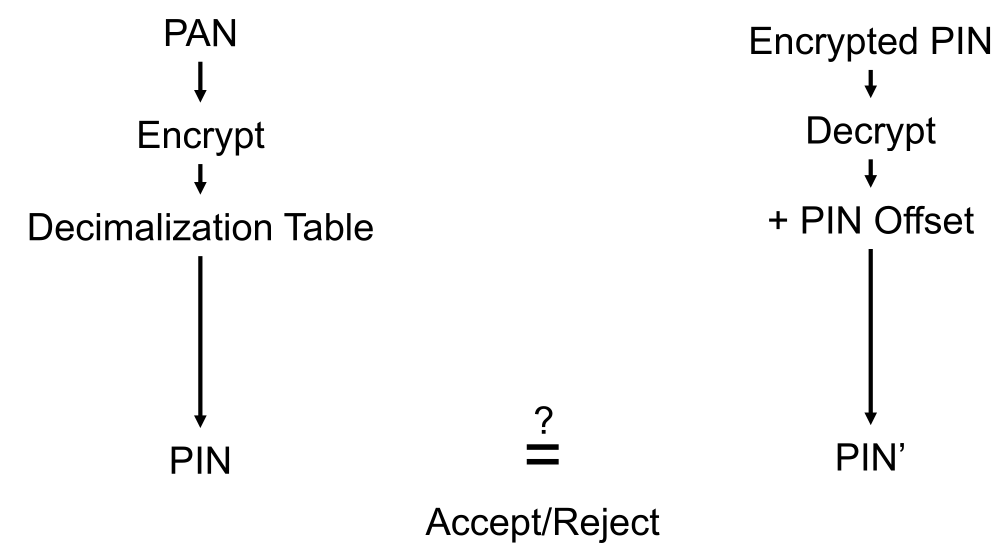
\includegraphics[width=0.6\columnwidth]{tamper_resilience_PIN-attack.png}
\end{center}

\subsubsection{Chip and PIN}
Man in the middle attack:
\begin{center}
  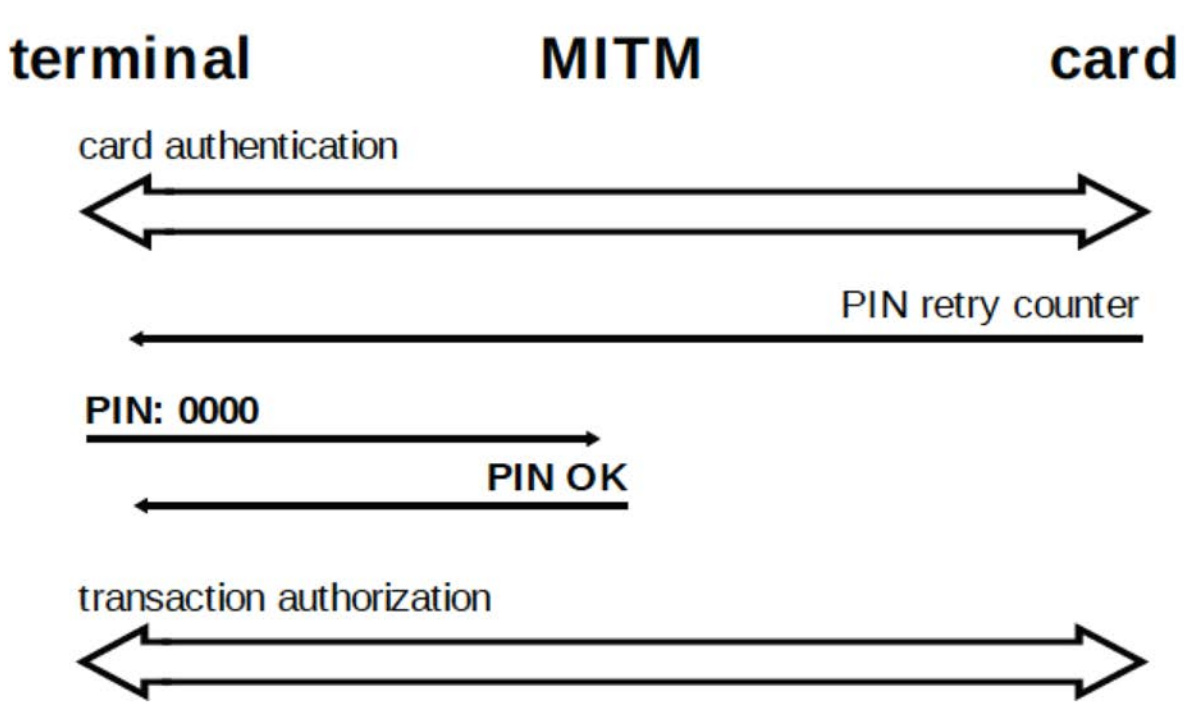
\includegraphics[width=0.5\columnwidth]{tamper_resilience_chip-and-pin.png}
\end{center}
Before the transaction, the MITM tells card that transaction will be signed on
paper $\Rightarrow$ No PIN required.

\subsection{Protection}
\begin{itemize}
  \item Access Control
  \item Limit functionality
    \begin{itemize}
      \item E.g. Do not allow other decimalization tables
    \end{itemize}

\end{itemize}
